    \documentclass{article}

% if you need to pass options to natbib, use, e.g.:
%     \PassOptionsToPackage{numbers, compress}{natbib}
% before loading neurips_2019

% ready for submission
% \usepackage{neurips_2019}

% to compile a preprint version, e.g., for submission to arXiv, add add the
% [preprint] option:
%     \usepackage[preprint]{neurips_2019}

% to compile a camera-ready version, add the [final] option, e.g.:
\usepackage[]{neurips_2019}

% to avoid loading the natbib package, add option nonatbib:
%     \usepackage[nonatbib]{neurips_2019}

\usepackage[utf8]{inputenc} % allow utf-8 input
\usepackage[T1]{fontenc}    % use 8-bit T1 fonts
\usepackage{hyperref}       % hyperlinks
\usepackage{url}            % simple URL typesetting
\usepackage{booktabs}       % professional-quality tables
\usepackage{amsfonts}       % blackboard math symbols
\usepackage{nicefrac}       % compact symbols for 1/2, etc.
\usepackage{microtype}      % microtypography
\usepackage{authblk}
\usepackage{graphicx}
\title{News Recommendation Engine}

\author[1]{Ankita Pal\thanks{A.apal1994@uw.edu}}
\author[1]{Chavi Gupta\thanks{B.chavig@uw.edu}}
\author[1]{Medha Sagar\thanks{C.sagarme@uw.edu}}
\affil[1]{Department of Data Science, University of Washington}

\renewcommand\Authands{ and }

\begin{document}
\maketitle

\begin{abstract}
    The goal of this project is to build a News Recommender System. We chose to work on a News Recommender system since we were interested in addressing both the dimensionality (associated with large text content) and recommendation problems that were covered in class. Among the different domains of recommender systems, news recommendation has been explored relatively less due to the lack of structured data and features. Text mining for news articles using NLP techniques in itself is a different class of problem. In this project we aim to build a pipeline for extracting user and news article features, and eventually build a hybrid recommender system to address the problems of cold start, data sparcity and scalability. 
\end{abstract}

\section{Introduction}

{Thorough introduction of your problem}

\section{Relevant Work}


\section{Data Collection}

{Description of the data collection process}

\section{Exploratory Data Analysis}

{Description of any initial findings or summary statistics from your dataset}

\section{Algorithm}

\begin{figure}
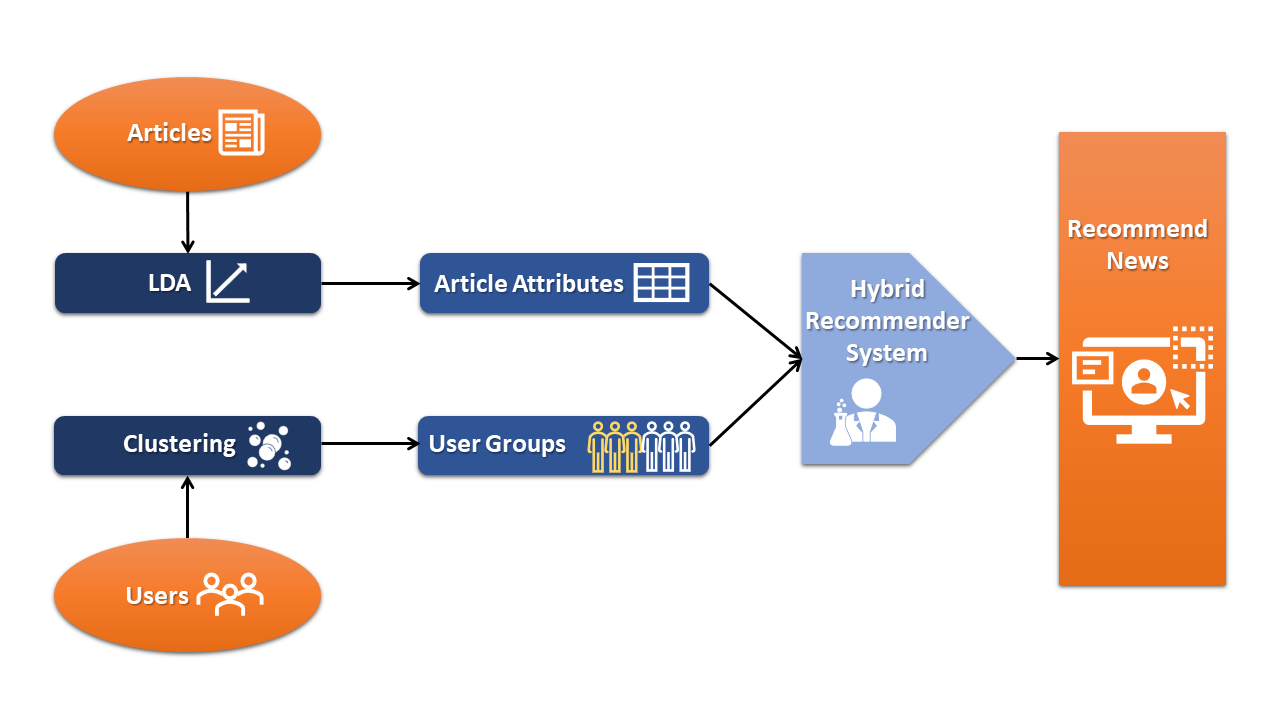
\includegraphics[scale=.40]{NeuRIPS2019/Slide1.PNG}
\caption{Workflow}
\end{figure}

\subsection{Article profiling using LDA}

\subsection{User profiling using Clustering}

\subsection{Hybrid CF-CBF Algorithm for News Recommendation}

\section{Conclusion}

{Description of general difficulties with your problem which bear elaboration
}

\begin{thebibliography}{9}

\bibitem{litReview} Çano, E.,\& Morisio, M.\ (2017). Hybrid recommender systems: A systematic literature review. {\it Intelligent Data Analysis}, 21(6), 1487-1524.
\end{thebibliography}
\end{document}
